\section{Chapter 10 Experimental Design and Evaluation Plan}

\subsection{10.1 Introduction}

This chapter presents the experimental design and evaluation methodology proposed for validating the effectiveness of the CloudSentinel AI framework. The objective of the experimental evaluation is to determine whether the proposed framework improves cloud security assessment when compared with existing Cloud Security Posture Management (CSPM) solutions. The evaluation focuses on four key aspects:

\begin{itemize}
\tightlist
\item
  Accuracy of cloud misconfiguration detection\\
\item
  Identification of multi-stage attack paths\\
\item
  Effectiveness of context-aware risk prioritization\\
\item
  Quality and usefulness of AI-generated security explanations
\end{itemize}

The overall evaluation workflow is illustrated in Figure 10.1, showing the sequence from cloud environment preparation to comparative analysis.

\begin{figure}[H]
\centering
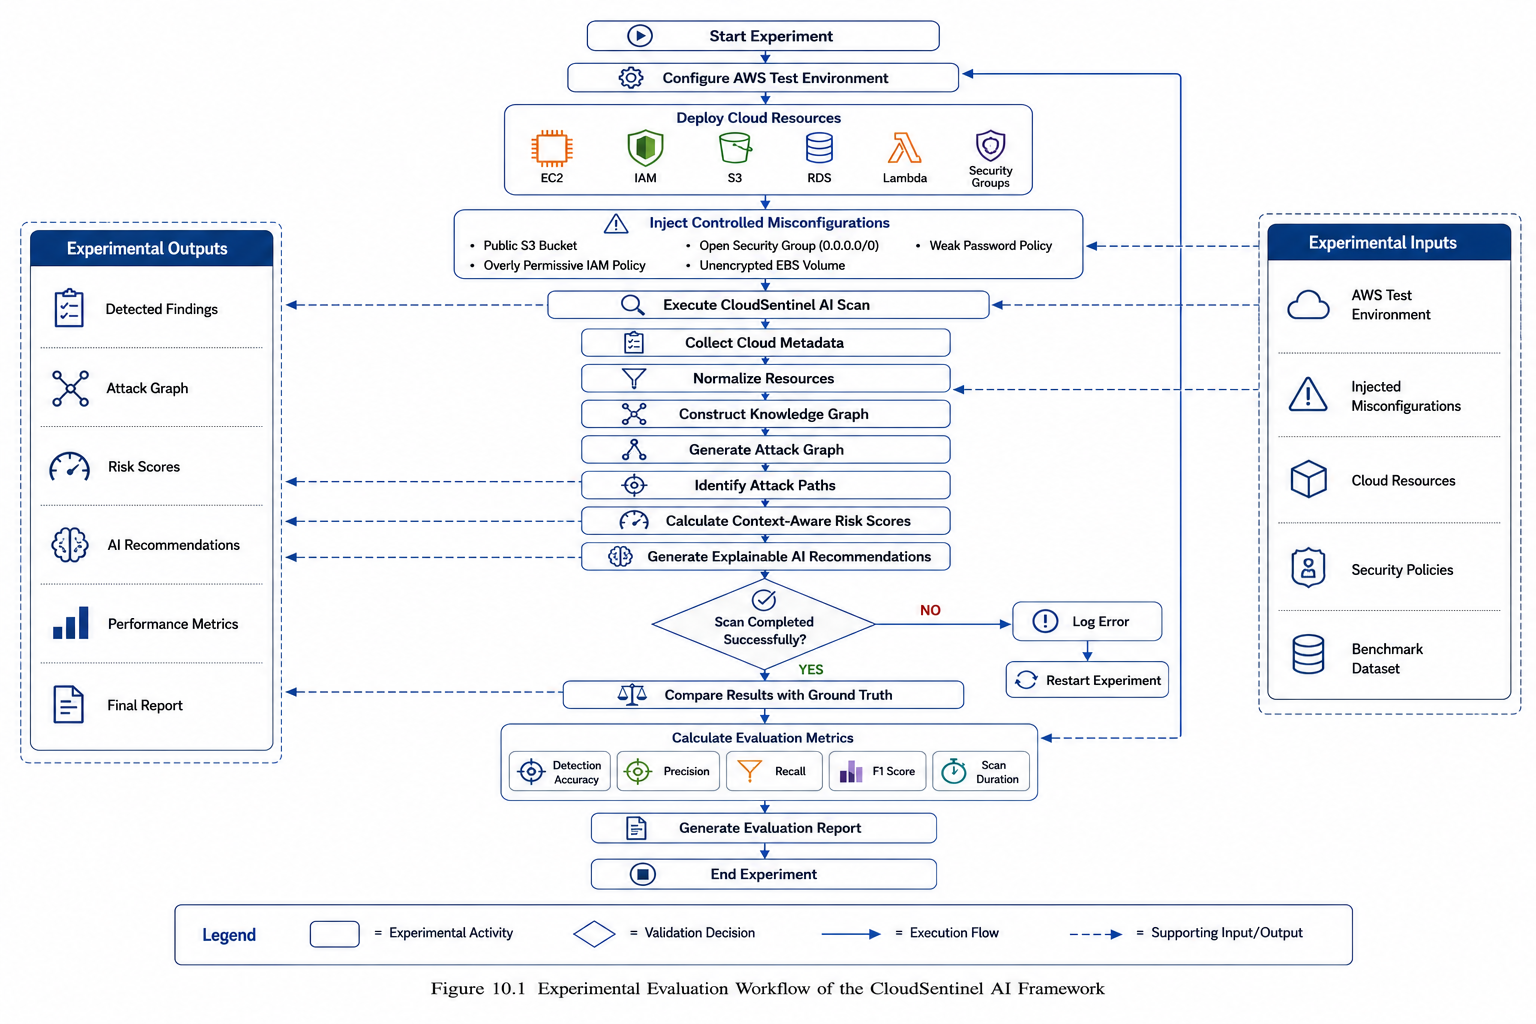
\includegraphics[width=0.9\textwidth,height=\textheight]{figures/image-10.1.png}
\caption{Experimental Evaluation Workflow.}\label{fig:10_1}
\end{figure}

\subsection{10.2 Experimental Objectives}

The experiments are designed to evaluate the proposed framework against predefined research objectives.

\begin{itemize}
\tightlist
\item
  \textbf{Objective 1:} Evaluate the ability of CloudSentinel AI to identify cloud misconfigurations across AWS resources.\\
\item
  \textbf{Objective 2:} Measure the framework's capability to generate realistic attack paths by correlating multiple cloud resources.\\
\item
  \textbf{Objective 3:} Assess the effectiveness of contextual risk scoring compared to static severity classifications.\\
\item
  \textbf{Objective 4:} Evaluate the quality and interpretability of AI-generated security explanations.\\
\item
  \textbf{Objective 5:} Compare the overall performance of CloudSentinel AI with selected baseline cloud security tools.
\end{itemize}

\subsection{10.3 Experimental Environment}

All experiments will be conducted in a controlled Amazon Web Services (AWS) environment to ensure reproducibility and minimize external influences.

\begin{longtable}[]{@{}ll@{}}
\toprule\noalign{}
Component & Specification \\
\midrule\noalign{}
\endhead
\bottomrule\noalign{}
\endlastfoot
Cloud Platform & Amazon Web Services (AWS) \\
Operating System & Ubuntu Linux \\
Programming Language & Python \\
Backend Framework & FastAPI \\
Graph Library & NetworkX \\
Database & PostgreSQL \\
Container Platform & Docker \\
Version Control & GitHub \\
\end{longtable}

\subsection{10.4 Experimental Scenarios}

To evaluate the framework under realistic conditions, several cloud environments with intentionally introduced security weaknesses will be created.

\begin{itemize}
\tightlist
\item
  \textbf{Scenario 1 -- Public Storage Exposure:} Amazon S3 buckets will be configured with public read or write permissions. Expected Outcome: Detect public bucket, sensitive data exposure, business impact, and remediation recommendation.\\
\item
  \textbf{Scenario 2 -- Overly Permissive IAM Policies:} IAM users and roles will be assigned excessive administrative privileges. Expected Outcome: Identify privilege escalation risks, excessive permissions, and potential attack paths.\\
\item
  \textbf{Scenario 3 -- Insecure Network Configuration:} Security Groups will intentionally expose SSH and RDP ports to the Internet. Expected Outcome: Detect internet-facing resources, network exposure, and possible attack chains.\\
\item
  \textbf{Scenario 4 -- Disabled Logging:} AWS CloudTrail logging will be disabled. Expected Outcome: Identify reduced visibility, explain the impact on forensic investigations, and recommend enabling centralized logging.\\
\item
  \textbf{Scenario 5 -- Multi-Stage Attack Chain:} A realistic attack chain will be constructed by combining a public EC2 instance, weak Security Group, excessive IAM permissions, access to AWS Secrets Manager, and sensitive S3 bucket. Expected Outcome: Generate a complete attack graph demonstrating how an attacker could move from the exposed EC2 instance to sensitive data.
\end{itemize}

\subsection{10.5 Baseline Tools for Comparison}

To evaluate the effectiveness of CloudSentinel AI, the experimental results will be compared with established cloud security tools.

\begin{longtable}[]{@{}
  >{\raggedright\arraybackslash}p{(\columnwidth - 8\tabcolsep) * \real{0.2000}}
  >{\raggedright\arraybackslash}p{(\columnwidth - 8\tabcolsep) * \real{0.2000}}
  >{\raggedright\arraybackslash}p{(\columnwidth - 8\tabcolsep) * \real{0.2000}}
  >{\raggedright\arraybackslash}p{(\columnwidth - 8\tabcolsep) * \real{0.2000}}
  >{\raggedright\arraybackslash}p{(\columnwidth - 8\tabcolsep) * \real{0.2000}}@{}}
\toprule\noalign{}
\begin{minipage}[b]{\linewidth}\raggedright
Tool
\end{minipage} & \begin{minipage}[b]{\linewidth}\raggedright
Misconfiguration Detection
\end{minipage} & \begin{minipage}[b]{\linewidth}\raggedright
Attack Path Analysis
\end{minipage} & \begin{minipage}[b]{\linewidth}\raggedright
Context-Aware Risk
\end{minipage} & \begin{minipage}[b]{\linewidth}\raggedright
Explainable AI
\end{minipage} \\
\midrule\noalign{}
\endhead
\bottomrule\noalign{}
\endlastfoot
AWS Security Hub & \(\checkmark\) & \(\times\) & Limited & \(\times\) \\
AWS Config & \(\checkmark\) & \(\times\) & \(\times\) & \(\times\) \\
Prowler & \(\checkmark\) & \(\times\) & \(\times\) & \(\times\) \\
ScoutSuite & \(\checkmark\) & Partial & \(\times\) & \(\times\) \\
CloudSentinel AI & \(\checkmark\) & \(\checkmark\) & \(\checkmark\) & \(\checkmark\) \\
\end{longtable}

\subsection{10.6 Evaluation Metrics}

The performance of CloudSentinel AI will be assessed using quantitative and qualitative evaluation metrics.

\subsubsection{10.6.1 Detection Metrics}

\begin{itemize}
\tightlist
\item
  Number of discovered resources\\
\item
  Number of detected misconfigurations\\
\item
  Detection coverage\\
\item
  False Positive Rate (FPR)\\
\item
  False Negative Rate (FNR)
\end{itemize}

\subsubsection{10.6.2 Performance Metrics}

\begin{itemize}
\tightlist
\item
  Asset discovery time\\
\item
  Configuration analysis time\\
\item
  Knowledge graph construction time\\
\item
  Attack graph generation time\\
\item
  Context-aware risk assessment time\\
\item
  Total execution time\\
\item
  CPU utilization\\
\item
  Memory consumption
\end{itemize}

\subsubsection{10.6.3 Attack Path Metrics}

\begin{itemize}
\tightlist
\item
  Number of generated attack paths\\
\item
  Average attack path length\\
\item
  Reachability between critical assets\\
\item
  Critical attack chains identified
\end{itemize}

\subsubsection{10.6.4 Risk Prioritization Metrics}

\begin{itemize}
\tightlist
\item
  Accuracy of prioritization\\
\item
  High-risk asset identification\\
\item
  Reduction in low-value alerts\\
\item
  Consistency of contextual scoring
\end{itemize}

\subsubsection{10.6.5 Explainable AI Metrics}

\begin{itemize}
\tightlist
\item
  Clarity of explanations\\
\item
  Completeness of recommendations\\
\item
  Technical accuracy\\
\item
  Readability for security analysts\\
\item
  Actionability of remediation guidance
\end{itemize}

\subsection{10.7 Experimental Workflow}

\begin{enumerate}
\def\labelenumi{\arabic{enumi}.}
\tightlist
\item
  Deploy the AWS test environment with predefined configurations.\\
\item
  Introduce controlled cloud misconfigurations for each experimental scenario.\\
\item
  Execute CloudSentinel AI to collect cloud assets and identify security issues.\\
\item
  Construct the knowledge graph representing cloud resources and their relationships.\\
\item
  Generate attack paths based on graph traversal and detected vulnerabilities.\\
\item
  Calculate contextual risk scores for each attack path.\\
\item
  Generate AI-assisted explanations and remediation recommendations.\\
\item
  Execute baseline tools under identical conditions.\\
\item
  Compare results using the selected evaluation metrics.\\
\item
  Analyze the findings and summarize the performance of the proposed framework.
\end{enumerate}

\subsection{10.8 Data Analysis Strategy}

The collected experimental data will be analyzed using descriptive statistics and comparative analysis. This includes comparison of detection rates, attack path identification, contextual risk prioritization effectiveness, execution times, and usefulness of AI-generated explanations.

\subsection{10.9 Threats to Validity}

\begin{itemize}
\tightlist
\item
  \textbf{Internal Validity:} Test environments may not represent every real-world AWS deployment.\\
\item
  \textbf{External Validity:} The initial implementation focuses on AWS; results may differ for Azure, Google Cloud Platform, or hybrid environments.\\
\item
  \textbf{Construct Validity:} Risk scores depend on the contextual factors selected for evaluation.\\
\item
  \textbf{Conclusion Validity:} Performance measurements may vary with hardware specifications, cloud environment size, and network conditions.
\end{itemize}

\subsection{10.10 Expected Outcomes}

CloudSentinel AI is expected to detect misconfigurations with high accuracy, generate meaningful multi-stage attack paths, prioritize risks effectively, reduce alert fatigue, and provide clear, actionable AI-generated explanations.

\subsection{10.11 Chapter Summary}

This chapter presented the experimental design and evaluation plan for validating the CloudSentinel AI framework. It defined the objectives, environment, scenarios, baseline tools, metrics, workflow, data analysis strategy, and threats to validity, establishing a structured approach for validating the research.

\subsection{Additional Figures}

\begin{figure}[H]
\centering
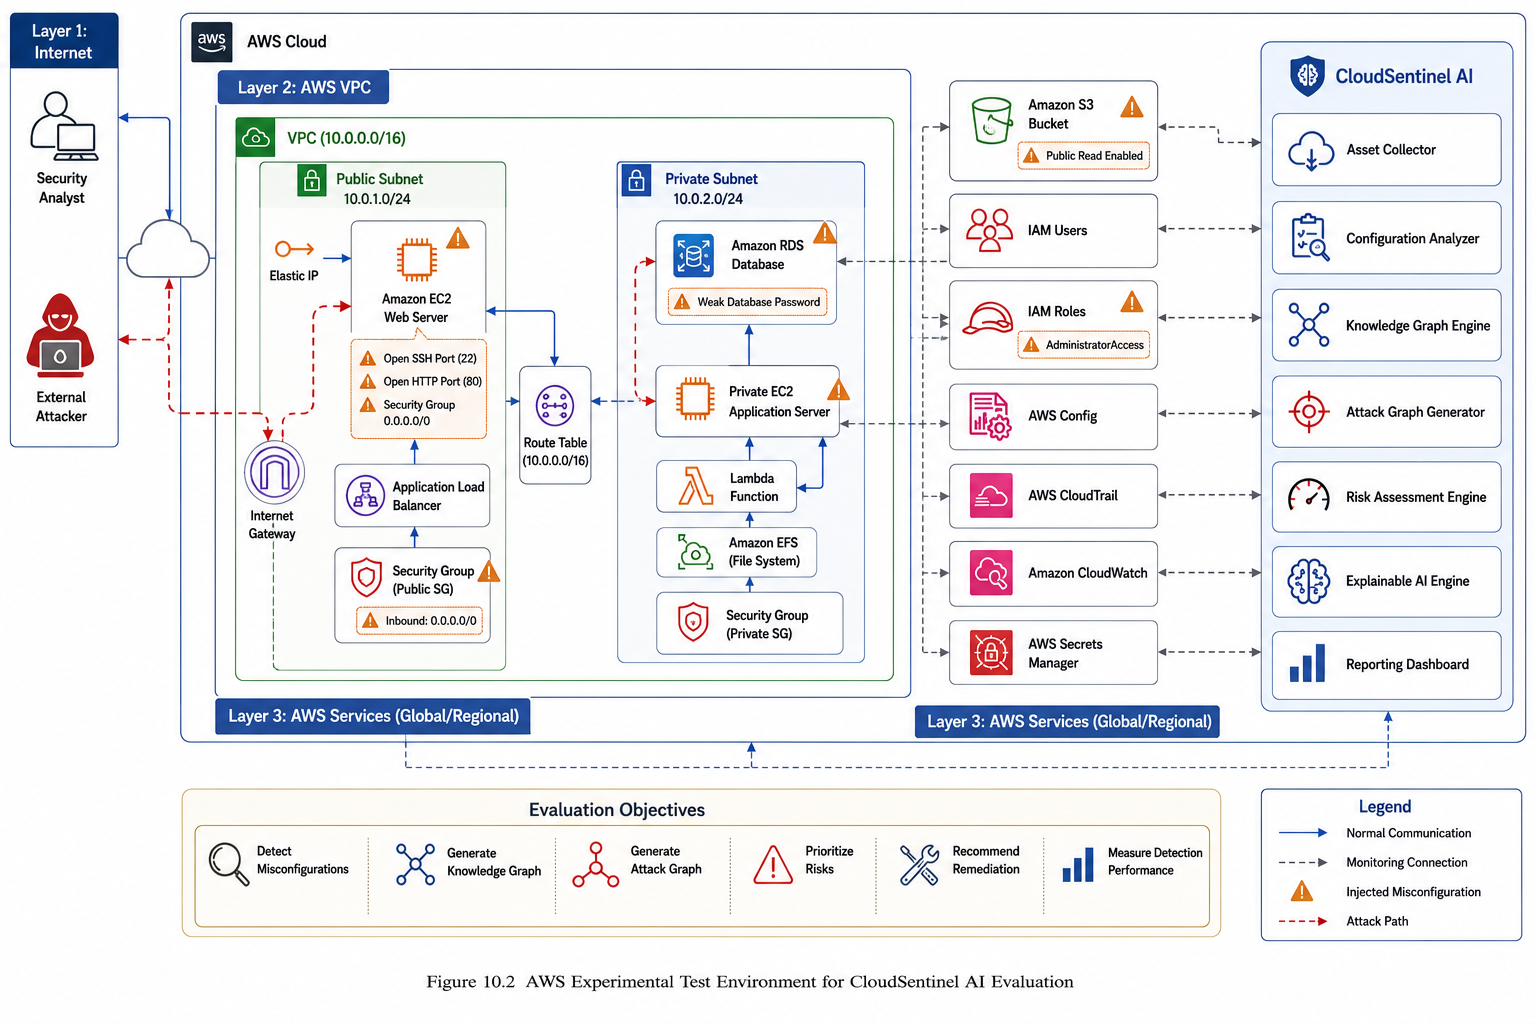
\includegraphics[width=0.9\textwidth,height=\textheight]{figures/image-10.2.png}
\caption{Injected Misconfiguration Scenario Design.}\label{fig:10_2}
\end{figure}

\begin{figure}[H]
\centering
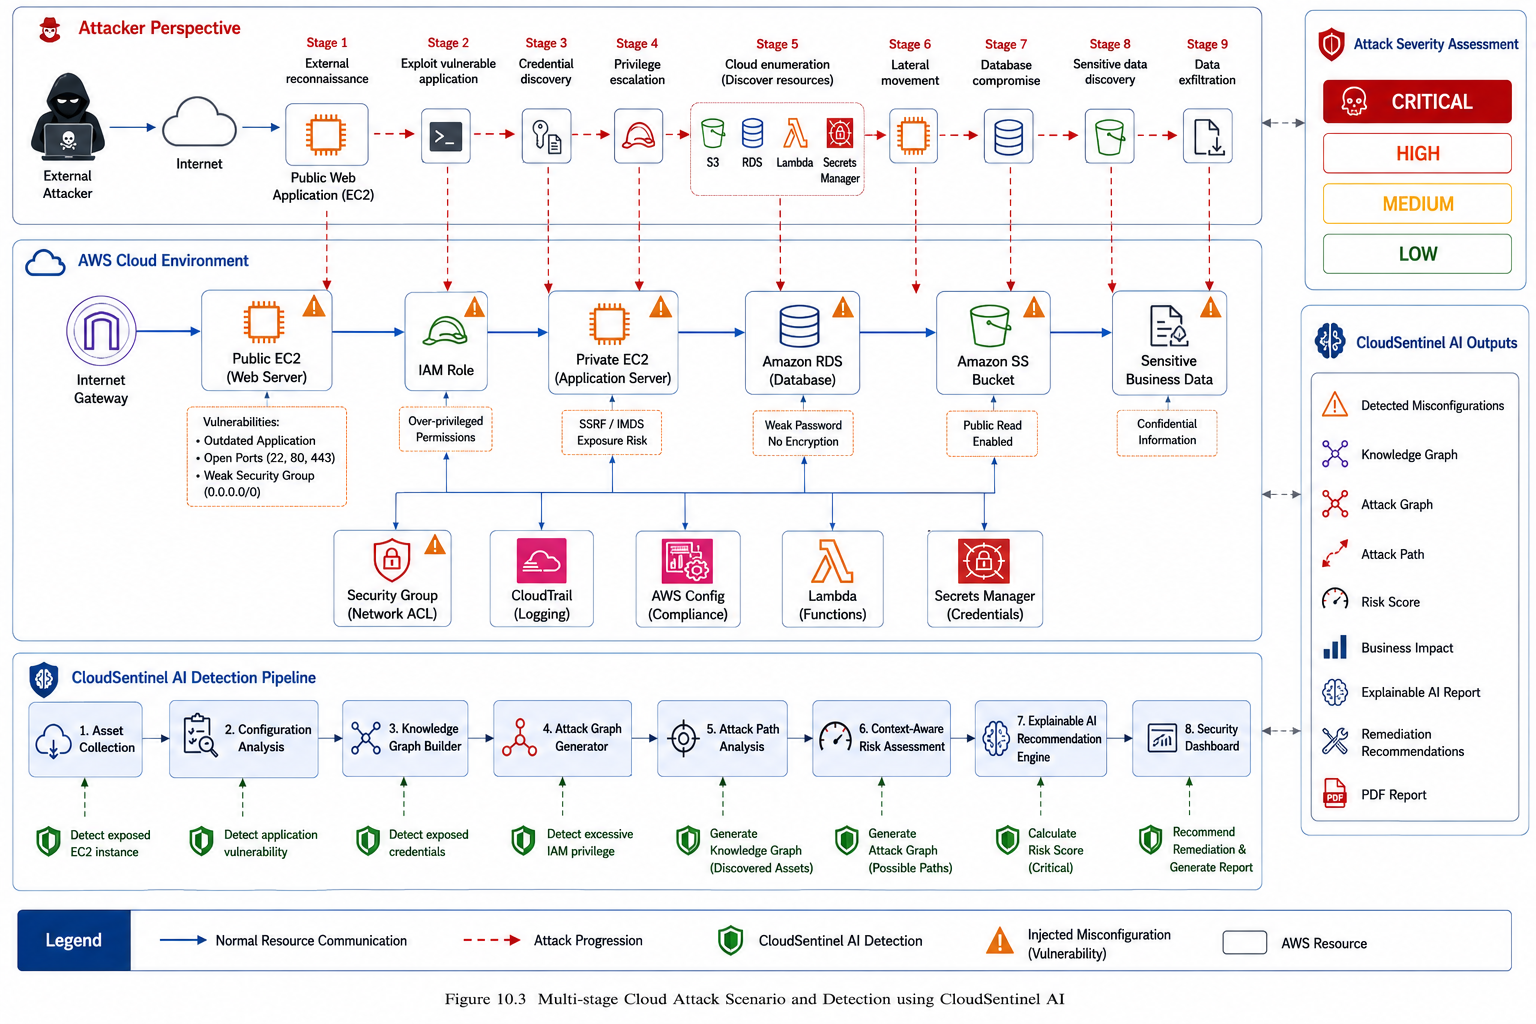
\includegraphics[width=0.9\textwidth,height=\textheight]{figures/image-10.3.png}
\caption{Evaluation Metrics and Analysis Flow.}\label{fig:10_3}
\end{figure}

\begin{figure}[H]
\centering
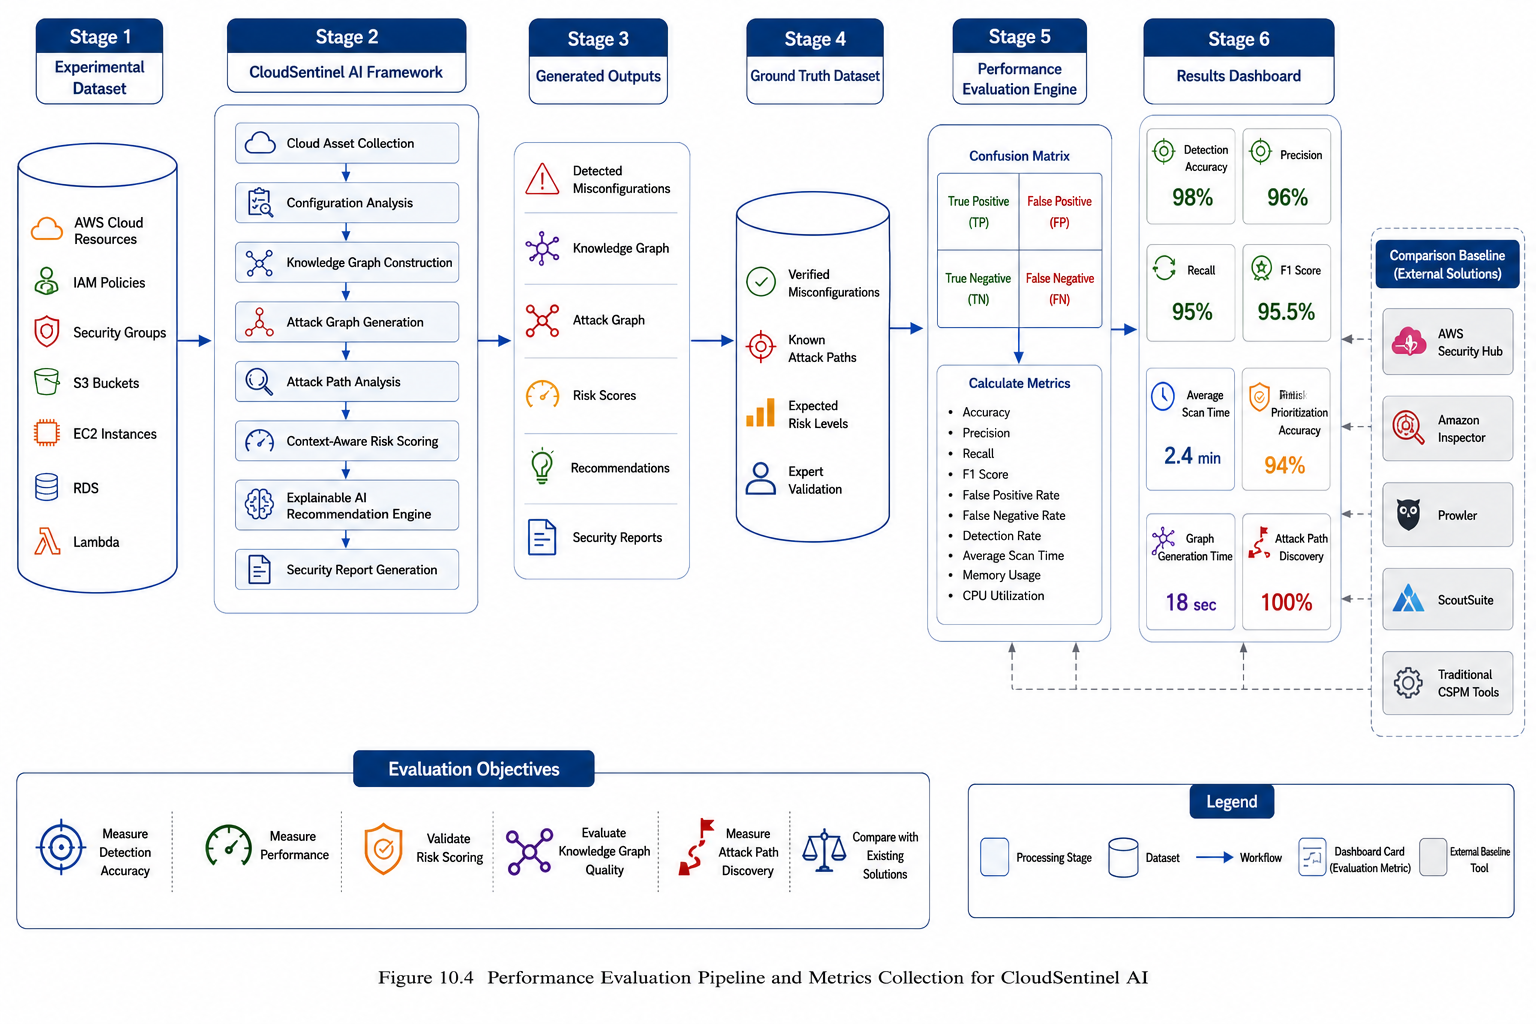
\includegraphics[width=0.9\textwidth,height=\textheight]{figures/image-10.4.png}
\caption{End-to-End Validation Scenario.}\label{fig:10_4}
\end{figure}
